%!TEX root = ../dissertation.tex
\begin{savequote}[75mm]
The only problem with testing ETH is you need another copy of the Universe to interfere with!
\qauthor{Professor Markus Greiner}
\end{savequote}

\chapter{Isolated quantum systems and \newline local thermalization within eigenstates}
\label{sec:ch4}

Having discussed entanglement and correlation properties in the context of equilibrium systems in the previous section of this thesis, we will now focus on the development of these properties in a pure, isolated quantum non-equilibrium system. The system's non-equilibrium dynamics will be used to probe the nature of its excited eigenstates. We will see that these excited eigenstates also have a generic, local behavior with characteristic dynamics that identify these eigenstates as belonging to a non-equilibrium quantum phase.

\section{Quantum thermalization}

When an isolated quantum system is strongly perturbed, for example by a sudden change in the Hamiltonian (a so-called quantum quench), the ensuing dynamics are determined by the population of eigenstates in the final Hamiltonian after the quench:\cite{Sakurai1993} at any given time, the evolving quantum state will have amplitudes that depend only on the eigenstates populated by the quench, their respective phases, and their energy eigenvalues in the final Hamiltonian. In many cases, such a system would be difficult to simulate exactly due the generation of a large amount of entanglement during the ensuing dynamics \cite{Calabrese2005,Amico2008,Daley2012,Schachenmayer2013}. Remarkably, however, the same isolated quantum system can locally thermalize under its own unitary dynamics -- unaided by an external reservoir -- meaning that the tools of statistical mechanics apply in describing the long-time, saturated behavior of the system \cite{Deutsch1991,Rigol2008,Eisert2015}. In this case, most local observables of a quantum state that is coherently evolving according to the Schr\"odinger equation can be predicted from a thermal ensemble and thermodynamic quantities. Even with infinitely many copies or realizations of this quantum state, these local observables are fundamentally unable to distinguish whether the global system is a single, many-body quantum state or a thermal ensemble. This statement is remarkably powerful: a globally pure quantum system is locally indistinguishable from a mixed, globally entropic thermal ensemble \cite{Jensen1985,Deutsch1991,Srednicki1994,Rigol2008}. The dynamic convergence of the pure quantum state via unitary evolution towards the predictions of a thermal ensemble and the entanglement that drives it are the focus of this chapter.

%\begin{figure}[ht!]
%		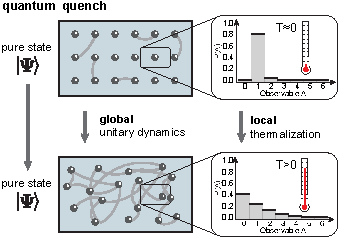
\includegraphics[width=3 in]{figures/ch4/fig1.pdf} 
%		\caption{\textbf{Conceptual Picture a,}  }
%		\label{fig:eth}	
%\end{figure}

\begin{figure}
\floatbox[{\capbeside\thisfloatsetup{capbesideposition={right,top},capbesidewidth=3 in}}]{figure}[\FBwidth]
{\caption{\textbf{Quantum thermalization.} The characteristic thermalizing behavior of our closed quantum system is probed via a quantum quench. The system initially starts at equilibrium with both a global and local entropy that is approximately zero. The system is then strongly perturbed by a sudden change in the Hamiltonian. As the system evolves only under its unitary evolution, it comes to a local equilibration that is indistinguishable from that of a globally entropic ensemble even though it is verifiably still part of a globally pure quantum state. This local agreement with a thermal ensemble is mediated by the growth of entanglement with the remaining system and generates local entropy.} \label{fig:eth}}
{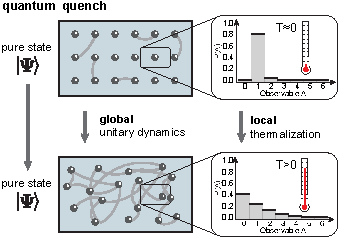
\includegraphics[width=3 in]{figures/ch4/fig1.pdf}} 
\end{figure}

Many theoretical studies have helped clarify the role quantum mechanics plays in statistical physics \cite{Deutsch1991, Rigol2008, Jensen1985, Srednicki1994, Santos2012, Deutsch2013, DAlessio2016}. The questions surrounding the agreement of local observables in pure quantum many-body states with extensively entropic thermal distributions are resolved by the implications of quantum entanglement in the pure state. The generation of local entropy by ignoring parts of a globally pure quantum system is the conceptual glue that connects how a pure quantum state can appear locally like a thermal ensemble. The key point is that this local entropy does not derive as some fraction of the globally entropic system. Rather, it originates from the ignoring of the quantum correlations shared between the local subsystem and the remainder of the full system.

\section{Protocol and Model}
\label{sec:ch4protocol}

The work presented in this chapter directly measures the global purity of a thermalizing quantum system through quantum many-body interference\cite{Daley2012,Islam2015,Kaufman2016}. We experimentally verify that a globally pure quantum state dynamically loses local purity to entanglement, and, in parallel becomes locally thermal. Other recent experiments have demonstrated aspects of quantum thermalization through the relationship between classical chaotic dynamics and entanglement in a superconducting qubit system\cite{Neill2016} and the dynamics of thermalization within an ion system \cite{Clos2016}.

All quench experiments are initialized from a $2\times6$ size plaquette of a larger low-entropy Mott insulator with unity filling (Fig.~\ref{fig:eth_protocol}\textbf{a}). The separability of the Mott insulator implies that the entire state is initialized as a product state of single-atom Fock states on each lattice site. This separability allows us to think of the $2\times6$ size plaquette as two copies of identical $1\times6$ site systems. The subsequent dynamics of this system will be given by a two-dimensional Bose-Hubbard Hamiltonian shown below:

\begin{equation}
\label{eqn:hjx}
\hat{H} = -(J_x \sum_{x,y} \hat{a}^\dagger_{x,y} \hat{a}_{x+1,y} + J_y \sum_{x,y} \hat{a}^\dagger_{x,y}\hat{a}_{x,y+1} + h.c. ) + \frac{U}{2} \sum_{x,y} \hat{n}_{x,y} (\hat{n}_{x,y}-1)
\end{equation}

As illustrated pictorially in Fig.~\ref{fig:eth_protocol}\textbf{a}, the quench dynamics are initiated by suddenly switching on the tunneling in the $x$ direction, whereas tunneling in the $y$ direction remains suppressed. These dynamics are restricted to a one-dimensional 6-site chain for both copies. This quench realizes a projection of the initial state onto many highly excited energy eigenstates in the final Hamiltonian. Each chain represents an identical and independent copy of a quenched system of six particles on six sites, which evolves in the quenched Hamiltonian for a variable duration. At the end of this evolution time, the dfynamics are frozen and one of the two protocols depicted in Fig.~\ref{fig:eth_protocol}\textbf{c} is performed. To measure the local occupation number on each site of the copy, we perform a one-dimensional time-of-flight measurement along the $y$ direction while a barrier remains between the two copies. To measure the global and local purity of the system, the tunneling along the $y$ direction between the two copies is rapidly increased to realize a many-body--interference measurement as mentioned in \S $\ref{sec:ch3}$ \cite{Islam2015}. Two examples of such results are shown in Fig.~\ref{fig:eth_protocol}\textbf{c} for both the local on-site occupation statistics and the global many-body purity.

\begin{figure}[t!]
		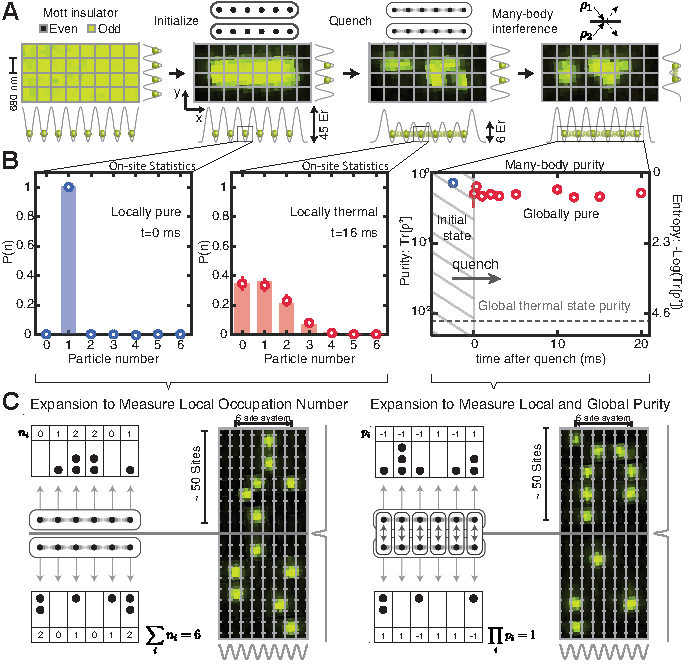
\includegraphics[width=\columnwidth]{figures/ch4/fig2_protocol.pdf} 
		\caption{\textbf{Protocol. a)} The experimental protocol starts with a unity filled Mott insulator, from which a $2\times6$ plaquette is sliced out with the installed DMD. The thermalizing unitary dynamics is realized by a sudden quantum quench of the lattice depth down to $6\mathrm{Er}$. The system is then either imaged in a site-resolve, number-sensitive fluorescence scheme shown in \textbf{c} or a many-body--interference operation is performed on the system to obtain the global and local purities of the system (shown in \textbf{c}). \textbf{b)} The resultant local on-site distributions are shown for the very non-thermal initial state and the thermalized quenched state. The global purity is plotted on the far right to demonstrate how unitary the dynamics are in preserving the global purity (red) of the initial state (blue). \textbf{c)} The two final protocols are shown here: the left) demonstrates a time-of-flight technique used to expand the one-dimensional systems into an orthogonal dimensions such that they may be imaged while avoiding parity projection; the right) demonstrates the same readout protocol after having performed the many-body--interference operation.}
		\label{fig:eth_protocol}	
\end{figure}

The ability to verify the quantum purity and presence of entanglement in the studied quantum many-body state is crucial for discerning the role of entanglement in the system. Fundamentally, the two-copy interference technique used directly provides access to observables that are quadratic in the density matrix and hence to the system's local and global purity\cite{Islam2015}. Other techniques to extract this quantity, such as quantum-state tomography, would be particularly challenging due to the large size of the full 462-dimensional Hilbert space defined by the itinerant particles in the system. 

\section{Non-equilibrium systems and highly excited eigenstates}
\label{sec:ensPredict}

Much of our conceptual understanding about the link between entanglement entropy and the expected thermal entropy of an ensemble\cite{Santos2012,Deutsch2013} is provided by the eigenstate thermalization hypothesis (ETH) \cite{Deutsch1991,Rigol2008,Jensen1985,Srednicki1994}. ETH provides an explanation for how closed quantum systems come to local agreement with a globally entropic thermal ensemble and is often framed in terms of the small variation of observables associated with eigenstates that are close in energy\cite{Deutsch1991,Rigol2008,Srednicki1994}. The role of entanglement in the eigenstates is paramount to this agreement\cite{Deutsch2013}. Fundamentally, the ETH implies an equivalence of the local, reduced density matrix of a single excited energy eigenstate and the local reduced density matrix of a globally thermal state \cite{Nandkishore2015}.\footnote{Conceptually, this  single eigenstate acts as the minimal version of a microcanonical ensemble and resembles the traditional equilibrium frameworks.} This equivalence is made possible only by entanglement and the local entropy it induces locally within a globally pure state.  

Since we cannot experimentally populate a single, excited eigenstate in the system, we do not probe how the ETH applies at the single eigenstate level. Instead, we perform a quench (Fig.~\ref{fig:eth_protocol}) which brings the global system far from equilibrium and study the unitary dynamics of the many excited eigenstates populated by this quench. However, since these eigenstates all individually are thermal according to ETH and vary slowly from eigenstate to eigenstate with energy, the quantum average over this superposition of states provide a qualitatively similar result to the single eigenstate.

We examine the presence of thermalization by performing a series of measurements of local observables and comparing them to thermal predictions of various ensembles. The eigenstate distribution resulting from a quench, Fig.~\ref{fig:statMech}\textbf{a}, determines the resulting dynamic values of the observables and their subsequent saturated values. Importantly, the final values of the Hamiltonian are $U/J_x < (U/J)_c$ where $(U/J)_c$ is the critical point in the superfluid-to-Mott-insulator transition. This is relevant because the eigenstates below this transition point are known to be non-integrable and therefore can be ergodic within global thermodynamic constraints. The underlying explanation for the ETH is that these excited eigenstates in the thermalizing, non-integrable system are nearly like random vectors or, equivalently, are described by a Hamiltonian that is described by random matrix theory \cite{Deutsch1991,DAlessio2016}. The diffuse probability distribution of eigenstates in most bases, in this case the Fock state basis, is analogous to the chaotic dynamics of a closed classical mechanical system that passes through all allowed points of phase space. This chaotic eigenstate assumption, like in the classical system, can be adapted to explain the saturated valeus of measured local observables, agreement of these saturated values with thermal ensembles, and the presence of a volume law in the entanglement entropy \cite{Deutsch1991,DAlessio2016, Page1993, Hyungwon2014Th}. The distinction between the classical and quantum cases is that the classical case experiences chaos in its temporal dynamics which realizes both entropy maximization and thermalization as a time-averaged effect. While in the quantum case, these characteristics are directly encoded into the properties of nearly every individual excited energy eigenstate.

In Fig.~\ref{fig:statMech}\textbf{c} \& \textbf{d}, we compare our measurements to the predictions of several thermal ensembles as illustrated in Fig.~\ref{fig:statMech}\textbf{b}. We also compare our results to a grand-canonical ensemble truncated to our total atom number (see Appendix: \ref{appendix:Ch4Cal}). The grand-canonical ensemble most closely models how well the many-body state can act as a reservoir for its constituent subsystems. For both the single-site and three-site subsystem observables, we show the atom number distributions for two different effective temperatures: $T=3.8J$ and $T=11J$. These effective temperatures are achieved by the final quench parameters of the Hamiltonian to $J/U=0.64$ and $J/U=2.6$ respectively. The effective temperature is determined by matching the average energy of the quench system with the calculated average energy originating from the population of the global energy eigenstates by a canonical ensemble at temperature $T$.

\begin{figure}[t!]
		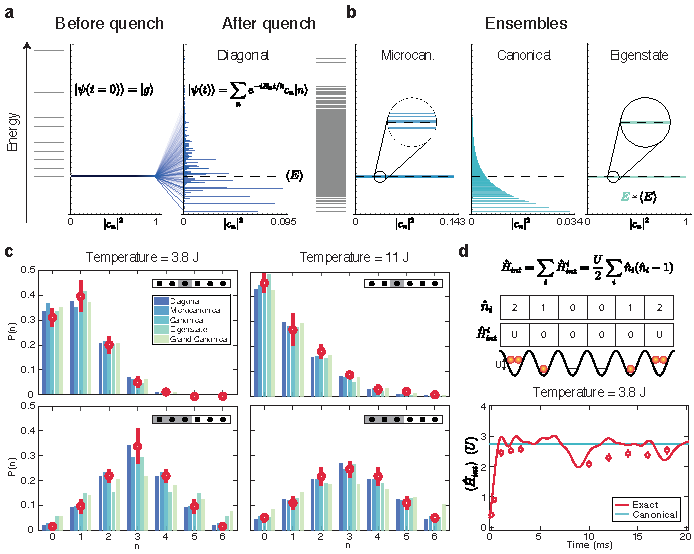
\includegraphics[width=\columnwidth]{figures/ch4/fig6_Ensemble_Figure.pdf} 
		\caption{\textbf{Statistical mechanical ensembles. a)}  The quantum quench populates the initial state across many of the eigenstates in the final Hamiltonian. \textbf{b)} We compare the results of our dynamics to several statistical ensembles: a microcanonical ensemble of a few eigenstates closest to the average global energy, the canonical ensemble where the temperature is chosen such that it has the same average energy, and a single eigenstate in the limit where we take the microcanonical ensemble to admit only the closest eigenstate to the average energy. \textbf{c)} The number distributions are plotted as a function of subsystem size and statistical ensemble prediction. \textbf{d)} The average interaction energy of the full state, a relatively global observable, is also plotted as a function of time which also agrees with the thermal prediction. All data are averaged in the saturated regime $10-20\mathrm{ms}$. error bars are the s.e.m. Eigenstates are found by exact diagonalization.}
		\label{fig:statMech}	
\end{figure}

For the smallest subsystem considered, the single site, the data are in good agreement with all ensembles considered. This conceptually agrees with our intuition as well since the single site can use all of the remaining system as an effective bath with which to share information and become locally thermal. Remarkably, despite the fact that the quenched state is a large distribution of eigenstates, our data show agreement with a microcanonical ensemble\footnote{This wording is a bit confusing since a single eigenstate is by definition not an ensemble. However, we use this terminology to relate to the language of statistical mechanical ensembles in the limiting case that a microcanonical ensemble admits only a single eigenstate.} consisting of a single eigenstate which is chosen to be the eigenstate with the closest energy to the average. This illustrates the key principle of the ETH; the reduced density matrix and its associated observable values vary slowly from eigenstate to eigenstate and are therefore relatively insensitive to the width of the distribution of populated states from the quench. This agreement between the ensembles and the measured values is relatively good even up to the subsystems of half the system size. The enhanced deviation hints at the fact that this larger sub-system is more sensitive to the fact that the global system is not truly a thermal ensemble.

%Trace Distance:
%
%\[
%T(\rho_A) = \frac{1}{2} \mathrm{Tr} \left ( |\rho^T_A - \rho_A| \right )
%\]
%
%Fidelity:
%
%\[
%F(\rho_A) = \mathrm{Tr} \left ( \sqrt{\sqrt{\rho^T_A} \rho_A \sqrt{\rho^T_A}} \right )
%\]
%
%\begin{figure}[ht!]
%		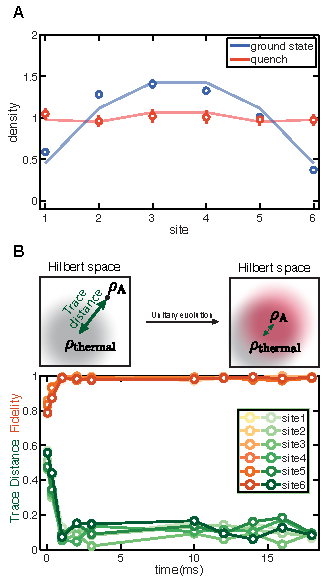
\includegraphics[width=3 in]{figures/ch4/fig5_fidelity_and_density.pdf} 
%		\caption{\textbf{Fidelity a,}  }
%		\label{fig:ss_fid}	
%\end{figure}

Since the above measurements rely on the full Fock-state read out, this technique allows for the extraction of other global observables (Fig.~\ref{fig:statMech}\textbf{d}). Since  the interaction term is diagonal in the measured basis (\ref{eqn:hjx}), our measurements allow the computation of the expectation value of the interaction energy $\left \langle \hat{H}_{int} \right \rangle = \left \langle \frac{U}{2} \hat{n}_i (\hat{n}_i-1) \right \rangle$. For the $T=3.8J$ data, we show a time series of both the initial growth of this quantity after the quench and its long-time agreement with the canonical prediction. Since this measurement is sensitive to the entire six-site system, it might at first glance seem to be sensitive to the global state purity and be unlikely to agree with thermalization. However, $\left \langle \hat{H}_{int} \right \rangle$ indeed thermalizes because it is a sum of local operators that all agree with thermal predictions and are insensitive to the global purity of the full system. This observation emphasizes that only a small number of global operators, such as global purity, are sensitive enough to truly distinguish the globally pure state from a thermal one.

\section{Entropy from entanglement and thermalization}

While the above results and predictions by the ETH provide a relationship between local predictions of single eigenstates and thermal ensembles, they do not provide any intuition for how the remainder of the system acts as a functional bath. To answer this question, we study the dynamics of entanglement entropy immediately after the quench for a variety of subsystem sizes (Fig.~\ref{fig:ee_dyn}). Initially, we observe a rapid and approximately linear rise in the entropy with time with a similar slope among all considered subsystems (Fig.~\ref{fig:ee_dyn} inset) \cite{Calabrese2005}. After a subsystem-size-dependent evolution time, the entanglement entropy saturates to a steady-state value, about which there are small residual temporal fluctuations. The origin of these small residual temporal fluctuations is the finite size of the system. 

\begin{figure}[t!]
		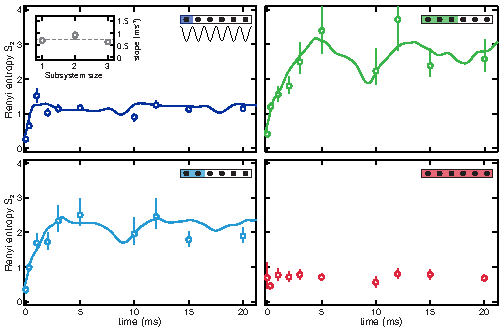
\includegraphics[width=\columnwidth]{figures/ch4/fig3_ee_dynamics.pdf} 
		\caption{\textbf{Entanglement entropy dynamics and saturation.} The second-order R\'enyi entropy is plotted for three different subsystem sizes as a function of evolution time. Both the time necessary for saturation scales and the fluctuations about the saturated value scale with the system size. The global entropy, plotted in the bottom right (red), remains substantially lower than all the measured local entropies and therefore satisfies that the local entropy is indeed due to entanglement. All error bars are the s.e.m. The solid lines are determined by exact diagonalization with an additional offset added due to extensive classical entropy as measured by the global entropy. }
		\label{fig:ee_dyn}	
\end{figure}

These observed entanglement entropy dynamics agree well with exact numerical calculations with no free parameters. The data show how the considered subsystems acquire entropy with time even though, crucially, the system as a whole retains only a finite, time-independent entropy that is smaller than the subsystem entropies. The high purity of the global system proves that the dynamical increase in entropy in the subsystems originates in the production of entanglement between the system's constituents. Furthermore, in analogy to the growth of thermodynamic entropy in an equilibrating classical mechanical system, such as a gas in a closed container, we observe the growth of local entropy in a closed quantum mechanical system. The distinction being that in the quantum mechanical case, the mechanism for generating this entropy is through entanglement throughout the global system.

When a system thermalizes, we expect that the saturated values of local observables should correspond to the predictions of a statistical ensemble.  By analogy, if the entanglement entropy plays the role of thermal entropy in these ensembles, then in a thermalized pure state, we expect extensive growth in the entanglement entropy with subsystem volume. The linear scaling of the entanglement entropy with the volume of the subsystem being considered is commonly referred to as a volume law. In the case of the studied one-dimensional system this volume is defined by the length of the subsystem considered. Theoretical work using conformal field theory has shown that for quenched, infinite, continuous systems the long time entanglement entropy should follow a volume law \cite{Calabrese2004,Calabrese2005,Eisert2010}. This differs from the ground state entropy scaling considered in the previous chapter (\S \ref{sec:ch3}) which follows an area law \cite{Vidal2003,Calabrese2004,Calabrese2005,Eisert2010}. Characterizing the large amount of entanglement associated with such a volume law scaling is challenging because it results from  small but important contributions of entanglement from many of the available degrees of freedom in a given subsystem.

We observe that the measured entanglement entropy shows a near-volume law behavior with subsystem size. A linear growth with volume in the entanglement entropy occurs when the reduced density matrix of a subsystem incoherently populates a number of its states that approximately scales exponentially with the physical size. This is true for this system since the Bose-Hubbard model has a Hilbert space that scales approximately exponentially with the system size. This results in $S_2(A) = -log[\mathrm{Tr}(\rho_A^2)] \propto L_A$. While this scaling proportionality of a thermal system is robust, the exact slope of the scaling depends on the average energy of the thermalized pure state\cite{Vidmar2017,Garrison2018}.  

We can contrast this scaling behavior with the ground state by adiabatically reducing the lattice depth to the same final values as the quenched Hamiltonian. In the case of the superfluid ground state of the Bose-Hubbard model, the system is predicted to have an area law with logarithmically slow correction that depends on the subsystem size\cite{Calabrese2004}. These two cases are clearly distinguished by our measurements. The bending-over of the entanglement-entropy curve after the half-size subsystem indicates that the state is a globally pure one. Note that this entanglement-entropy curve additionally deviates at the half-size subsystem from the volume-law expectation. This deviation is expected as a result of random pure quantum states and is known as the Page correction \cite{Page1993}. 

\begin{figure}[t!]
		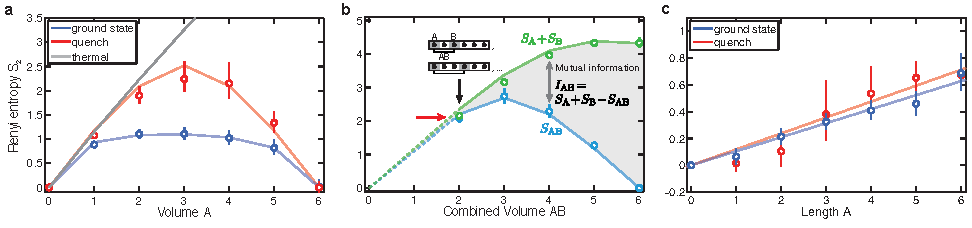
\includegraphics[width=\columnwidth]{figures/ch4/fig4_volumeLaw_edit.pdf} 
		\caption{\textbf{Scaling behavior. a)} The measured entanglement entropy is plotted as a function of considered subsystem size for both the thermalizing quenched state (red) and the equilibrium ground state (blue). The quenched state has entanglement scaling that qualitatively agrees with a volume and the predicted thermodynamic entropy (gray line). The ground state exhibits a scaling that is consistent with only an area law. Both curves must bend over at the mid point ($\mathrm{volume~A} = 3$) since they are both pure quantum states. \textbf{b)} In order to look for whether locally thermal systems appear independent,the mutual information between subsystems of sizes less than or equal to the total system size are compared. Once the combined system size is approximately half the system size, the subsystems begin to demonstrate their lack of independence. \textbf{c)} The measured extensive, classical entropy injected into the system during the experiment is determined by subtracting off the expected entanglement entropy from the measured values. The remaining entropy should reflect this truly classical entropy which appears to follow a true volume law up to the system size. The solid lines in \textbf{a,b} are calculated from exact diagonalization. The solid lines in \textbf{c} are from a linear fit. All error bars are the s.e.m.}
		\label{fig:volLaw}	
\end{figure}

%THING ABOUT PAGE CORRECTION SHOWN IN (ARXIV:1708.08453.pdf CITATION 34, OTHER NICE CITATIONS 29-33) look at vedika paper (I think critical one or 2 universality classes)

In the spirit of comparison between thermodynamic ensembles and the local properties of pure quantum states, we compare the measured entanglement entropy as a function of subsystem volume with the thermodynamic entropy predicted by a canonical thermal ensemble $\rho^T$ (where $T$ is the effective temperature and $\rho^T$ is determined the same way as written above). We find a near-quantitative agreement between the entanglement entropy and thermal entropy for a subsystem volume smaller than the half-system size. Unfortunately, the total system size limits this comparison to only a few points.

Despite their quantitative similarity, it is worth emphasizing the disparate character of the thermal and entanglement entropies. The entanglement entropy is an instantaneous quantity that is present in a pure state even for an infinitely precise measurement time. It arises from the non-separability of the quantum state between the subsystem and its traced-out degrees of freedom. This realizes an instantaneously truly classical ensemble. This differs in a fundamental way from the classical case. The von Neumann  entropy of a subsystem from a mixed thermal state is the thermodynamic entropy in statistical mechanics and can be extracted from irreversible heat flow experiments on the system \cite{Deutsch2013}. Additionally, from a physical point of view there is another important conceptual difference. At any given instant of time, a classical system resides in a well defined microstate and therefore would actually have zero entropy. Practically speaking however, no measurement is instantaneous and any such attempt to show this exact microstate would result in a time average that would provide the same thermodynamic prediction of a true instantaneous probability distribution. The quantum system, in some sense, actually provides a conceptually simpler picture for nature since the tracing out of any local subsystem will realize a truly mixed ensemble that is valid even instantaneously. 

This behavior of entanglement entropy not only provides a useful framework for describing thermalizing closed quantum systems, but also alleviates the need for the ad hoc statements for describing the behavior of classical ensembles. The quantum description encompasses the quantum properties we know to be true for isolated pure quantum systems and can also locally generate the classical properties we know phenomenologically to be true for classical thermodynamic systems. Remarkably, this also implies that one of the most well-known features of entanglement, the presence of non-local correlations, must somehow play a role in this behavior. In particular, the large amount of entanglement implied by the observed volume law suggests a large amount of correlations between disparate parts of the system, whereas a key feature of a thermal state is the absence of such long-range correlations. A useful metric for determining the amount of correlation between two subsystems, both classical and quantum, is the mutual information $I_{AB} = S_A + S_B - S_{AB}$ \cite{Wolf2008, Islam2015}. The mutual information in the presence of a volume law would find vanishing correlations between the two subsystem volumes, as would be the expectation for a thermodynamic statistical ensemble. Our data agrees with this prediction when the total volume considered is less than half the system size ($L_A+L_B\leq L/2$). This agreement breaks down once the total considered volume is a majority of the system size. There are additional bounds on the classically allowable mutual information described in \S $\ref{sec:ch3}$ that are violated in Fig.~\ref{fig:volLaw}\textbf{b}. This  demonstrates that while two local subsystems will agree with being uncorrelated, as predicted in the thermodynamic case, once their joint subsystem volume grows to encompass a majority of the system, the correlations related to the system being an entangled quantum state are revealed.

\section{Discussion}

These observations and measurements provide a natural link between thermalizing quantum mechanical systems and classical thermodynamic systems composed of itinerant particles. In fact, they allow for an interpretation of the known classical thermodynamic framework as a natural consequence of the quantum-mechanical behavior. They provide some of the justification for the necessary assumptions for classical statistical mechanics: a classical system in thermal equilibrium can be found in any microstate that is compatible with the thermodynamic constraints imposed on the system. The theoretical work related to the ETH demonstrates how this is true for the individual eigenstates of a thermalizing isolated quantum system. The ergodicity associated with exploring all available microstates is also justified even for instantaneous measurements by a quantum system and does not require time-averaging or multiple realizations of a system to generate a truly entropic ensemble \cite{DAlessio2016, Huang1963, Ma1985}. In fact, the superposition of states realizes a truly instantaneous, locally entropic ensemble that requires no additional statements.

This study hints at a microscopic origin for the maximization of entropy in a single quantum state. The ergodic nature of the eigenstates implies the system's entanglement is caused by scrambling correlations among all available degrees of freedom in the system. This scrambling of correlations is what realizes the thermal entropic scaling behavior when considering a small subsystem: a volume law occurs for small subsystem sizes since the amount of information (correlations) gained by including a larger subsystem is outweighed by the amount of new information lost among the all-to-all sharing of information. This fact is captured by the vanishing mutual information between subsystems whose joint volume is still small compared to the total system size.

These frameworks help establish the possibility for many-bodied classical behavior, namely statistical mechanics, to be interpreted as a subset of quantum-mechanical phenomena. The principles postulated classically out of practicality and physical agreement are now implied as the result of only resolving highly entangled quantum systems locally.\footnote{To put it bluntly, but not carefully, if the Universe were a non-integrable, interacting many-body quantum system in an excited but pure state, we would still realize a classical world on all practical human length scales.} While these eigenstate characteristics are not generically predicted for ground states, they are generically predicted for almost all excited eigenstates in itinerant, interacting many-body quantum systems that do not harbor some form of integrability that prevents ergodicity. In the next chapter we will study the only known robust exception to this phenomena, which is known as many-body localization\cite{Nandkishore2015,DAlessio2016}. This exception turns out to be the only known robust exception to the ETH paradigm and harbors excited eigenstates with characteristic behavior that appears to belong to another phase of eigenstates. This phase forms an extensive number of locally conserved quantities in the Hamiltonian that causes the ETH to fail and harbors unique entanglement dynamics \cite{Bardarson2012,Serbyn2013a,Serbyn2013b,Huse2014,Nandkishore2015}.